\documentclass[12pt,a4paper]{article}
\usepackage[utf8]{inputenc}
\usepackage{amsmath}
\usepackage{amsfonts}
\usepackage{amssymb}
\usepackage{makeidx}
\usepackage{graphicx}
\usepackage{lmodern}
\usepackage{color}
\usepackage{xcolor}
\usepackage{bussproofs}
\usepackage{lscape}
\usepackage{listings}
\usepackage{amsthm}
\usepackage{url}
\usepackage[left=2cm,right=2cm,top=2cm,bottom=2cm]{geometry}

\author{Mudathir Mahgoub}
\title{Symbolic Execution Engine}


\newtheorem*{remark}{\textbf{Remark}}

\begin{document}

\maketitle

\section {Project Problem}

Symbolic execution engines are commonly used in formal verification and software testing. Traditional testing methods use different input values to check specified properties about some code. Normally it is difficult to handle all possible input values especially when the input space is huge or infinite. Symbolic execution on the other hand relies on unknown symbolic values for the input and explores all possible execution paths while maintaining a symbolic state for each path. With the help of constraint solvers like SAT solvers or SMT solvers, we can reason about the specified properties and formally verify whether a property holds in all execution paths, or give a counter example if it doesn't. 

In this project the target code is a simple portion of the C programming language, and the properties are specified using assertions. 

\section{Motivation or Importance of the problem}

Symbolic execution is mostly used in software verification for critical systems. In such systems, strong security and safety properties need to be guaranteed. Examples of security properties include an array access within its range, and the absence of division by zero. An example of a safety property for software embedded in a microwave is guaranteeing that microwave is never running while its door is open. 

\subsection{Personal motivation}
Initially my idea was to do another project. When I was answering the last question in the take home exam it was about symbolic execution and the answer needed some constraints solving using high school math. After solving only 2 formulas, it became tedious and I tried to use z3 online to solve them. That also became more tedious to write SMT-LIB formulas, so finally I decided to do this project when the first project didn't work out. As a bonus I verified my manual answer to that question using this project. So for that I am satisfied. 

Another motivation is that symbolic execution is related to my research. So obviously this is supposed to be my first choice, but the first one involved reverse engineering which is really cool. Also I decided to use Z3 something different than CVC4 which I would be working on in the future. 
\section{Challenges} 

The paper \cite{paper} describes many challenges in symbolic execution that include:

\begin{itemize}
\item Scalability: exploring all execution paths doesn't scale well for large programs where number of paths increases exponentially. Therefore in large programs, mixing concrete execution with symbolic execution (concolic execution), and other heuristic approaches are usually used. 

\item Memory: how to symbolically execute operations on pointers, arrays, objects. In this project only variables are supported. 
\item Environment: how to symbolically interact with time, operating system, network. Environment is not supported in this project.
\item Loops: the number of paths depends on the number of iterations in the loop. In general, determining whether a loop terminates is not decidable. So symbolic execution can only work with restricted loops or use some heuristics. Loops are not supported in this project.
\item Constraint solving:  symbolic execution is limited by the power of the underlying solvers. For example non-linear arithmetic constraints, which are common, are not usually efficient in SMT solvers. 

\end{itemize}

\subsection{Project challenges}

Some issues arose during the implementation of the project. Here are some of them:

\begin{itemize}
\item A grammar for C: the official grammar is too much for this project, and many simple grammars in the internet were not enough. So I prepared a specific one with the help of 3 grammars 
cymbol\footnote{\url{https://github.com/remenska/Grammars/blob/master/book-examples/examples/Cymbol.g4}}, tinyC\footnote{\url{https://github.com/antlr/grammars-v4/blob/master/tinyc/tinyc.g4}}
and antlr C\footnote{\url{https://github.com/antlr/grammars-v4/blob/master/c/C.g4}} .  

\item  A grammar for SMT-LIB: the official grammar for SMT-LIB\footnote{\url{https://github.com/julianthome/smtlibv2-grammar/blob/master/src/main/resources/SMTLIBv2.g4}} is also a lot for this project which only uses integer arithmetic. So I wrote one just for parsing the counter examples returned by the SMT solver. 


\item Deadlock with Z3 process: one way to interact with Z3 is to call it as a separate process, and send SMT-LIB commands and receive the output. However Z3 process blocks waiting for an input when it executes the previous command. Initially the symbolic execution engine was implemented to send multiple commands and then receive the output of the satisfiablility checking or the model retrieval commands. This resulted in a deadlock where Z3 process is waiting for an input from the symbolic execution engine, and the engine is waiting for the output of Z3. Fortunately z3 supports the ``echo" command which I used to echo white space before reading the output of Z3. 

Another way to interact with Z3 is to use Z3 binding (e.g. com.microsoft.z3.jar for Java), however this approach makes it harder to use other SMT solvers like CVC4 with has its own Java binding (CVC4.jar). 
\end{itemize}

\section{Existing Approaches}

Paper \cite{paper} describes several approaches to symbolic execution including fully symbolic execution,  concolic execution, dynamic symbolic execution, selective symbolic execution, path selection, symbolic backward execution. It also describes many ways to handle memory including  fully symbolic memory, address concretization, partial memory modeling, lazy initialization. 

In this project I used fully symbolic execution with fully symbolic memory. 

\section{My approach}

A general overview of the project is given in section \ref{sec:software}. The symbolic execution engine is described in section \ref{sec:execution}.

\subsection{Software description} \label{sec:software}


\begin{figure}[h]
 \centering
 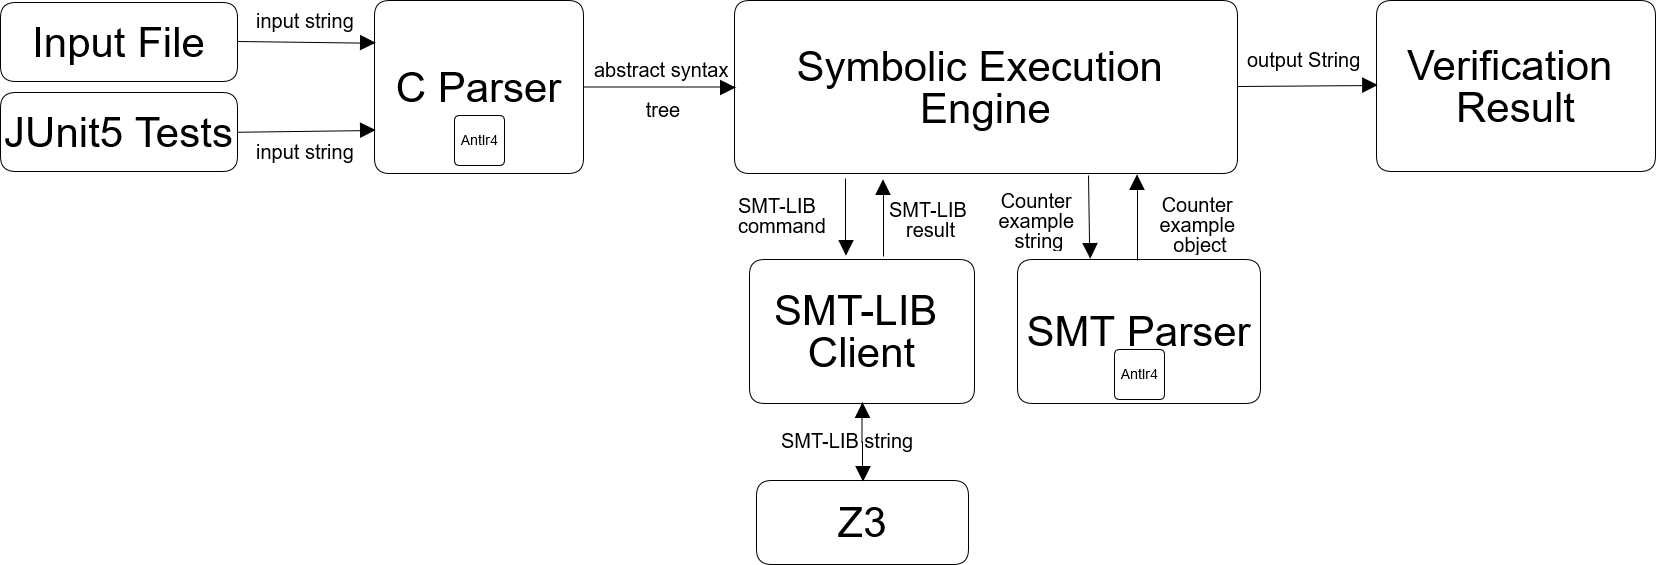
\includegraphics[scale=.25,keepaspectratio=true]{./engine.png}
 % gantt_chart.png: 0x0 pixel, 0dpi, nanxnan cm, bb=
 \caption{Project architecture.}
 \label{fig:engine}
\end{figure}

The project is implemented using Java and the executable is a jar file (target/SymbolicEngine.jar) which is generated using the command:
\definecolor{light-gray}{gray}{0.95}
\lstset{backgroundcolor= \color{light-gray}}

\begin{lstlisting}  
mvn install
\end{lstlisting}  

The program receives as an input a source file containing a simple C function. For testing, \textbf{JUnit5} was used to test the program directly using 45 unit tests. The input (from the input file or the unit test) is passed to the \textbf{C Parser} which uses the ANTLR library to parse the input into an abstract syntax tree. This abstract syntax tree is consumed by the \textbf{Symbolic execution engine} which executes statements and evaluates expressions symbolically to build assertion formulas which are encoded in SMT-LIB commands. These commands are passed to the \textbf{SMT-LIB client} which interacts with the SMT solver Z3.  
Z3 results are passed to \textbf{Symbolic execution engine} through \textbf{SMT-LIB Client}. Z3 counter examples are handled by the \textbf{SMT Parser}. Finally the \textbf{Symbolic execution engine} returns the verification results which include a validity answer for each formula: \textbf{Yes}, \textbf{No} with a counter example, or \textbf{Unknown}. 


Here is an example of an input:

\definecolor{light-gray}{gray}{0.95}

\lstset{caption={test.c},backgroundcolor= \color{light-gray}}


\begin{lstlisting}  
void f (int x, int y)
{
    if(x > 0)
    {
        y = x;
    }
    assert (y == x);
}
\end{lstlisting}

Here is the output:

\lstset{caption={java -jar SymbolicEngine.jar -i test.c}}

\begin{lstlisting} 
------------------
Overall Answer: No
------------------
Assertion: (BinaryExpression(Variable(y) == Variable(x)))
AssertionFormula:
(assert (> _x1 0))
(assert (not (= _x1 _x1)))
Answer: Yes
----------------------------
AssertionFormula:
(assert (not (> _x1 0)))
(assert (not (= _x2 _x1)))
Answer: No
Counter example: {x=0, y=1}
----------------------------

\end{lstlisting} 

The following section focuses on the symbolic execution engine. 

\subsection{Symbolic execution engine} \label{sec:execution}

The symbolic execution engine starts executing a function by symbolically assigning a new symbolic value to each argument variable. This would be the initial state of function and its block. The initial path constraint for the function would be the empty constraint (equivalent to $true$). For simplicity, I will just call the current state to mean both the current state and the current path constraint. 

For convenience each statement keeps track of \textbf{start states} where it can start from, and \textbf{end states} where it can end with. The \textbf{start states} of the current statement is exactly the \textbf{end states} of the previous statement. The block of a function has only one \textbf{start state} which is the one defined for the function. The first statement of each block inherits the \textbf{start states} of its block. Each statement can not modify its \textbf{start states}, but it can modify its \textbf{end states}. An assignment statement modifies each \textbf{start state} by updating the value of the variable changed in the assignment. A variable definition statement without an assignment would add that variable to the state with a new symbolic value. This is useful to reason about the following function:

\lstset{caption={},backgroundcolor= \color{light-gray}}

\begin{lstlisting}  
void f()
{
	int z;
	assert (z == z);
}
\end{lstlisting}

If the variable is defined with an assignment, the variable will be added to the state with value of the assigned expression. Only statements of assignments and variable definitions with assignment can modify a variable value in a state. Statements like (++i) or (i++) are rewritten as assignment statements (e.g. i = i + 1;)


Since loops are not supported, only \textbf{If statements} can modify path constraints in a state. The \textbf{If statement} will add its \textbf{condition} to the path constraint of each start state of its \textbf{true statement}. Likewise, the \textbf{If statement} will add the \textbf{negation of its condition} to the path constraint of each start state of its \textbf{false statement}. If the (\textbf{If statement}) has no \textbf{false statement}, it will be rewritten such that \textbf{NoOperation} statement is its \textbf{false statement} (similar to \textbf{nop} in assembly language). This is explained with the following example:

\begin{lstlisting}  
void f (int x, int y) 
{ 
	if(x > 0) y = x;  
	assert (y == x);
}
\end{lstlisting}

The above will be rewritten to be equivalent to 
\begin{lstlisting}  
void f (int x, int y) 
{ 
	if(x > 0) y = x;  
	else NoOperation();
	assert (y == x);
}
\end{lstlisting}

Whenever there is a division in an expression, the symbolic execution engine would automatically add an assertion statement such that the numerator of the division is not equal to zero. The \textbf{start states} of this assertion statement would be the \textbf{start states} of the statement where the division operation resides. This explained in the following example:

\begin{lstlisting}  
void f (int x, int y) 
{
	x = x / y;
}
\end{lstlisting}

The above would be rewritten to be equivalent to :

\begin{lstlisting}  
void f (int x, int y) 
{
	assert(y != 0);
	x = x / y;
}
\end{lstlisting}


Finally since C allows integers to be used as booleans in assertions, this would be problematical in Z3 which doesn't support that. Therefore assertions with integer expressions are written to be logical with comparison to zero as follows:

\begin{lstlisting}  
void f (int x, int y) 
{ 	
	assert (x+y);
	assert (0);
}
\end{lstlisting}

The above will be rewritten to be equivalent to 
\begin{lstlisting}  
void f (int x, int y) 
{ 	
	assert (x+y > 0);
	assert (0 > 0);
}
\end{lstlisting}

\section{Work Division} 

Since there is only one person in this project, all the work is done by him. 

\bibliographystyle{plain}

\bibliography{references}

\end{document}
